\documentclass[a4paper,11pt]{article}

\usepackage[utf8]{inputenc}
\usepackage[top=2cm, left = 2cm , right=2cm , bottom=2cm]{geometry}
\usepackage{amsmath}
\usepackage{graphicx}
\usepackage{float}
\usepackage{listings}
\usepackage[brazil]{babel}

\usepackage{color}

\definecolor{mygreen}{rgb}{0,0.6,0}
\definecolor{mygray}{rgb}{0.5,0.5,0.5}
\definecolor{mymauve}{rgb}{0.58,0,0.82}

\lstset{
  backgroundcolor=\color{white},   % choose the background color; you must add
                                   % \usepackage{color} or \usepackage{xcolor};
                                   % should come as last argument
  basicstyle=\footnotesize\sffamily,  % the size of the fonts
  breakatwhitespace=false,         % sets if automatic breaks should only happen
                                   % at whitespace
  breaklines=true,                 % sets automatic line breaking
  captionpos=b,                    % sets the caption-position to bottom
  commentstyle=\color{mygreen},    % comment style
  escapeinside={\%*}{*)},          % if you want to add LaTeX within your code
  extendedchars=true,              % lets you use non-ASCII characters; for
                                   % 8-bits encodings only, does not work with
                                   % UTF-8
  frame=single,	                 % adds a frame around the code
  keepspaces=true,                 % keeps spaces in text, useful for keeping
                                   % indentation of code (possibly needs
                                   % columns=flexible)
  keywordstyle=\color{blue},       % keyword style
  language=Matlab,                 % the language of the code
  numbers=left,                    % where to put the line-numbers; possible
                                   % values are (none, left, right)
  numbersep=5pt,                   % how far the line-numbers are from the code
  numberstyle=\tiny\color{mygray}, % the style that is used for the line-numbers
  rulecolor=\color{black},         % if not set, the frame-color may be changed
                                   % on line-breaks within not-black text
                                   % (e.g. comments (green here))
  showspaces=false,                % show spaces everywhere adding particular
                                   % underscores; it overrides
                                   % 'showstringspaces'
  showstringspaces=false,          % underline spaces within strings only
  showtabs=false,                  % show tabs within strings adding particular
                                   % underscores
  stepnumber=2,                    % the step between two line-numbers. If it's
                                   % 1, each line will be numbered
  stringstyle=\color{mymauve},     % string literal style
  tabsize=2,                       % sets default tabsize to 2 spaces
  title=\lstname                   % show the filename of files included with
                                   % \lstinputlisting; also try caption instead
                                   % of title
}

\pagestyle{plain}

\graphicspath{{./Imagens/}}

\begin{document}	

\begin{center}
\textbf{Pré-relatório Experiência 4} \\
\hspace{5pt}
Prof. Marconi Kolm Madrid \\
EA722 - 2017/2
\end{center}

\begin{center}
Danilo Pereira Titato - RA 122541 \\
Giovani Granzotto Oliani - RA 146253 \\
Pedro Gabriel Calixto Mendonça - RA 118363 \\
\end{center}

\textbf{1.}

\begin{gather*}
    k_i k_{hw} = 7500 \implies k_i = \frac{7500}{k_{hw}} \implies
        k_i = 0.5091
\end{gather*}

Para o caso criticamente amortecido, temos $k_p = 0.1191$, $k_d = 0.0093$.

\begin{figure}[H]
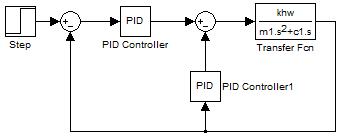
\includegraphics{q01-sistema}
\centering
\end{figure}

Simulando o sistema abaixo, com os $k_p$, $k_d$ e $k_i$ mencionados, sua
resposta ao degrau foi:

\begin{figure}[H]
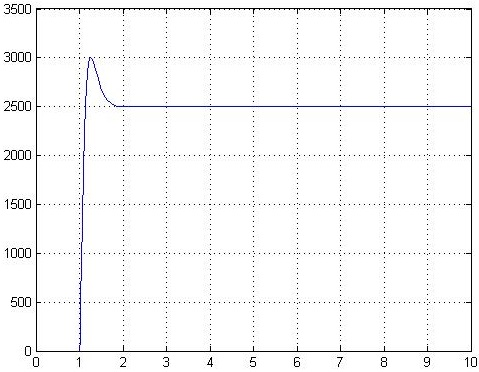
\includegraphics{q01-resp}
\centering
\end{figure}

\pagebreak

\textbf{2.} Dobrando o valor de $k_i$, temos como resposta:

\begin{figure}[H]
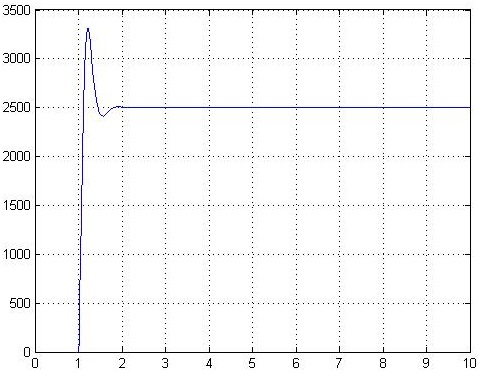
\includegraphics{q02-resp}
\centering
\end{figure}

Como podemos ver na resposta ao degrau, o aumento de $k_i$ não causou nenhuma
melhora no erro de regime, que já estava em zero na configuração anterior. Foi
causado um aumento visível no \textit{overshoot}. \\

\textbf{3.}

\begin{gather*}
    X_1\left(s\right) = \left[\left(R\left(s\right) - X_1\left(s\right)\right)
        \left(k_p + \frac{k_i}{s}\right) - k_d s X_1\left(s\right)\right]
        \frac{k_{hw}}{m_1 s^2 + c_1 s} \\
    X_1\left(s\right) = \left[R\left(s\right)
        \left(k_p + \frac{k_i}{s}\right) - X_1\left(s\right)
        \left(k_p + \frac{k_i}{s} + k_d s\right)\right]
        \frac{k_{hw}}{m_1 s^2 + c_1 s} \\
    X_1\left(s\right) \left[1 +
        \frac{\frac{k_{hw} \left(k_p + \frac{k_i}{s} + k_d s\right)}
        {m_1 s^2 + c_1 s}}{m_1 s^2 + c_1 s}\right] = \frac{\left[R\left(s\right)
        \left(k_p + \frac{k_i}{s}\right)\right] k_{hw}}{m_1 s^2 + c_1 s} \\
    \frac{X_1\left(s\right)}{R\left(s\right)} = 
        \frac{\left(k_p + \frac{k_i}{s}\right) k_{hw}}
        {m_1 s^2 + c_1 s + \left(k_p + \frac{k_i}{s} + k_d s\right) k_{hw}} =
        \frac{k_{hw} k_p s + k_{hw} k_i}
        {m_1 s^3 + \left(c_1 + k_{hw} k_d\right) s^2 + k_{hw} k_p s +
        k_{hw} k_i}
\end{gather*}

\pagebreak

Pólos e zeros do item 1:

\begin{figure}[H]
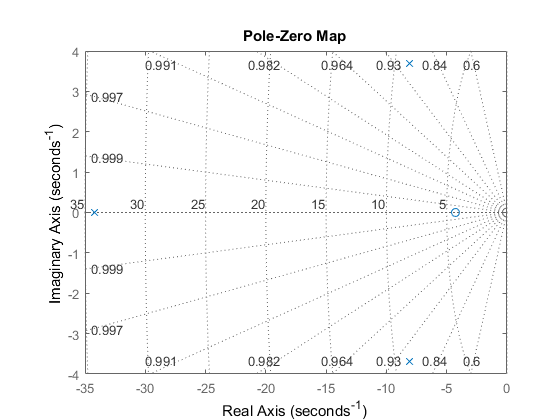
\includegraphics{q04-01}
\centering
\end{figure}

\begin{lstlisting}
p =
 -34.2295 + 0.0000i
  -8.0738 + 3.6996i
  -8.0738 - 3.6996i

z =
   -4.2746
\end{lstlisting}

\pagebreak

Pólos e zeros do item 2:

\begin{figure}[H]
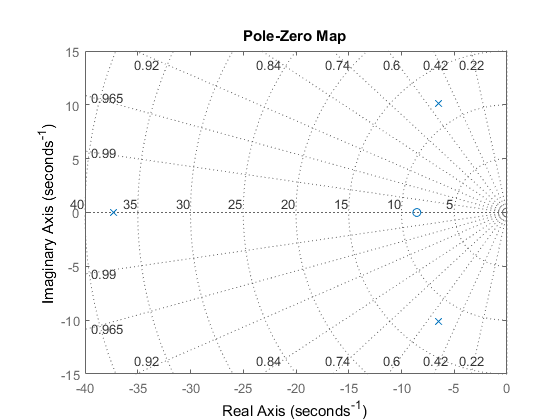
\includegraphics{q04-02}
\centering
\end{figure}

\begin{lstlisting}
p =
 -37.3334 + 0.0000i
  -6.5219 +10.1043i
  -6.5219 -10.1043i

z =
   -8.5491
\end{lstlisting}

\end{document}